\documentclass{article}

\renewcommand{\thesection}{\Roman{section}} 
\renewcommand{\thesubsection}{\thesection.\Roman{subsection}}
\renewcommand{\thesubsubsection}{\thesection.\thesubsection.\Roman{subsubsection}}
\newcommand{\horiline}{\noindent\rule{16cm}{0.4pt}}

\usepackage[letterpaper,top=2cm,bottom=2cm,left=3cm,right=3cm,marginparwidth=1.75cm]{geometry}
\usepackage[utf8]{inputenc}
\usepackage{enumitem}
\usepackage{amsmath} 
\usepackage{amsfonts}
\usepackage{mathtools} 
\usepackage{cancel}
\usepackage{tikz}
\usepackage{tkz-euclide}
\usepackage{caption}
\usepackage{graphicx}
\usepackage{xcolor}
\usepackage{bm}
\usepackage{float}
\usepackage{indentfirst}
\usepackage{csquotes}
\usepackage{tocloft}
\usepackage{hyperref}
\usepackage{tikz}
\usepackage{amsmath,mleftright,amssymb}
\usepackage{xparse}
\usepackage{pgfplots}
\usepackage{quiver}
\usepackage{pgffor}
\usepgfplotslibrary{fillbetween}    
\pgfplotsset{compat=1.8, width=10cm}
\usetikzlibrary{hobby,graphs,tikzmark,patterns,arrows.meta,decorations.pathreplacing,calc,positioning,shapes.geometric,backgrounds}
\pgfplotsset{compat=1.18}


\addtolength{\cftsecnumwidth}{10pt}
\setlength{\cftsubsecnumwidth}{30pt}
\setlength{\cftsubsubsecnumwidth}{40pt}

\DeclarePairedDelimiter\ceil{\lceil}{\rceil}
\DeclarePairedDelimiter\floor{\lfloor}{\rfloor}

\NewDocumentCommand{\evalat}{sO{\big}mm}{%
  \IfBooleanTF{#1}
   {\mleft. #3 \mright|^{#4}}
   {#3#2|^{#4}}%
}

\newcommand{\Li}[1]{\operatorname{Li_2}{\left(#1\right)}}

\usepackage{titletoc}% http://ctan.org/pkg/titletoc
\titlecontents*{chapter}% <section-type>
  [0pt]% <left>
  {}% <above-code>
  {\bfseries\chaptername\ \thecontentslabel\quad}% <numbered-entry-format>
  {}% <numberless-entry-format>
  {\bfseries\hfill\contentspage}% <filler-page-format>

\definecolor{tA}{RGB}{0,100,180}
\definecolor{tB}{RGB}{160,50,140}
\definecolor{tC}{RGB}{200,100,20}

\title{Holy Integrals}
\author{Zachary Medjamia}
\date{2026}

\begin{document}

\maketitle

\section*{Introduction}

This essay is devoted toward some of my favorite integral problems I've come across in the past (through books, forums, etc). I not only want to document them here but also provide some detailed insight and understanding behind each integral (not just their solutions). There's a few initial steps that we'll frequently use on every integral. We'll always start by plugging them directly into a calculator, I typically start with \href{https://www.integral-calculator.com/}{Integral-Calculator} and or \href{https://www.wolframalpha.com/}{WolframAlpha}. We'll also use an Inverse Symbolic Calculator (specifically RIES) to try and find a closed form solution using the numerical value of the integral. Also, feel free to try these integrals yourself before reading!

\section{$I_{0}$: Michael}
$$I_{0} = \int_{1}^{\sqrt{2}}{\frac{\arctan{\sqrt{2 - x^2}}}{1+x^2}dx}$$

\begin{center}
    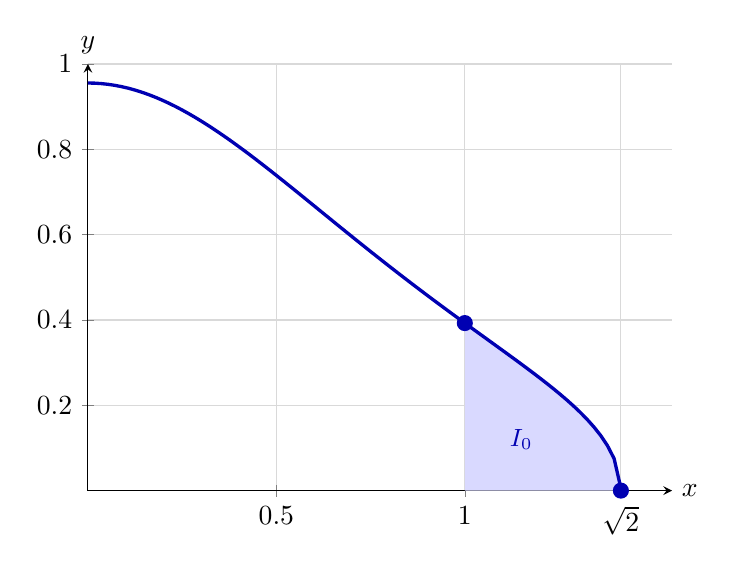
\begin{tikzpicture}
    \begin{axis}[
        at={(0,0)},
        width=9cm, height=7cm,
        xmin=0, xmax=1.55,
        ymin=0, ymax=1,
        xlabel={$x$},
        ylabel={$y$},
        axis lines=middle,
        xlabel style={at={(rel axis cs:1,0)}, anchor=west},
        ylabel style={at={(rel axis cs:0,1)}, anchor=south},
        xtick={0, 0.5, 1, 1.414},
        xticklabels={$0$, $0.5$, $1$, $\sqrt{2}$},
        ytick={0.2, 0.4, 0.6, 0.8, 1.0},
        grid=major,
        grid style={gray!30},
        samples=80,
        domain=0:1.4142,
        every axis plot/.append style={thick},
    ]
    % Shaded area
    \addplot[fill=blue!15, draw=none, domain=1:1.4142] {rad(atan(sqrt(2-x^2)))/(1+x^2)} \closedcycle;
    % Curve
    \addplot[blue!70!black, very thick, domain=0:1.4142] {rad(atan(sqrt(2-x^2)))/(1+x^2)};

    \addplot[only marks, mark=*, mark size=2.5pt, blue!70!black] coordinates {(1, 0.3927) (1.4142, 0)};

    \node[blue!70!black, font=\small] at (axis cs:1.15, 0.12) {$I_0$};
    \end{axis}
    \end{tikzpicture}
\end{center}

Using all the previously mentioned methods we've arrived at nothing (this is good!). Using the approximation numerical value of the integral: $0.1028083791780...$ (for the sake of intrigue I'll be using 100 digits), the RIES program returns
$$
\frac{(\arctan{1})^2}{6} = \frac{\left( \frac{\pi}{4} \right)^2}{6} = \frac{\pi^2}{96}
$$
as an exact match. Interestingly, the integral could be made equal to the area squared of a circle with radius $2\sqrt[4]{6}$. Occasionally, this process will allow us to possibly contemplate our next steps in solving. However, in this case, there isn't much motivation.

We can break up the integral by noticing $\arctan{\sqrt{2-x^2}} = \int_{0}^{\sqrt{2-x^2}}{\frac{1}{1+y^2}}dy$ as well as switching the order of integration while respecting the bounds to set up an interesting step,
\begin{align*}
\int_{1}^{\sqrt{2}}{\frac{\arctan{\sqrt{2 - x^2}}}{1+x^2}dx} &= \int_{1}^{\sqrt{2}}{\int_{0}^{\sqrt{2-x^2}}{\frac{1}{(1+x^2)(1+y^2)}dy}dx}\\ &= \int_{0}^{1}{\int_{1}^{\sqrt{2-y^2}}{\frac{1}{(1+x^2)(1+y^2)}dx}dy}
\end{align*}

The bounds makes more sense with a diagram

\begin{center}
    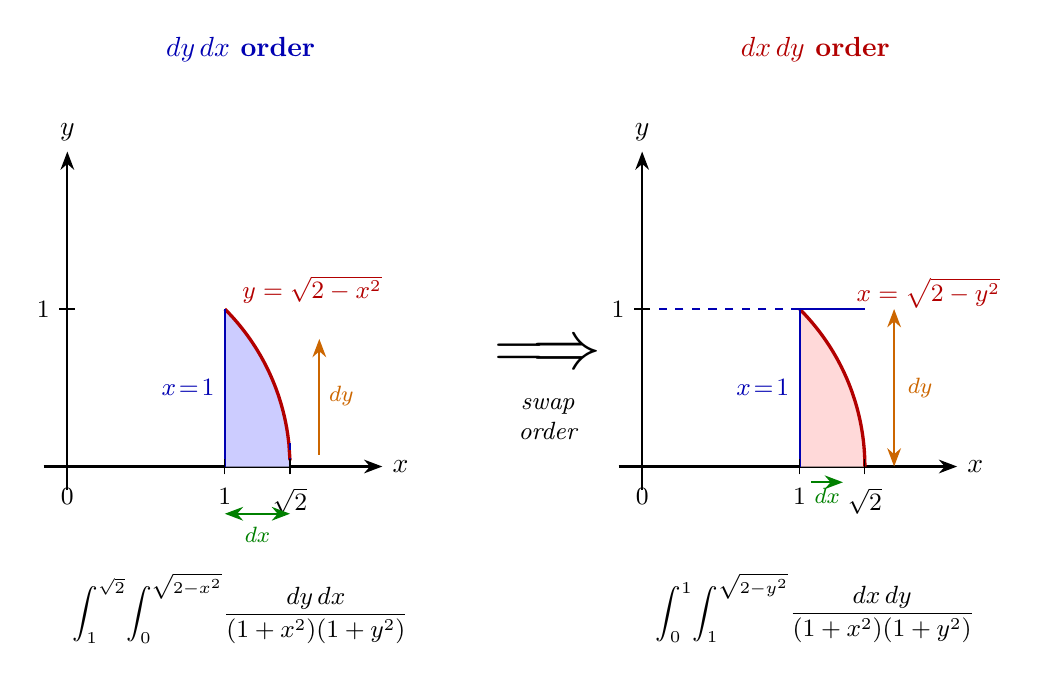
\begin{tikzpicture}
\begin{scope}[shift={(0.2,0.8)}]
\node[font=\bfseries, blue!70!black] at (2.2,5.3) {$dy\,dx$ order};

\draw[-Stealth, thick] (-0.3,0) -- (4,0) node[right] {$x$};
\draw[-Stealth, thick] (0,-0.3) -- (0,4) node[above] {$y$};

\begin{scope}
\clip (2,0) rectangle (2.828, 3);
\fill[blue!20] plot[domain=2:2.828, samples=60, variable=\x] ({\x},{sqrt(8-\x*\x)}) -- (2.828,0) -- (2,0) -- cycle;
\end{scope}

\draw[red!70!black, very thick, domain=2:2.828, samples=60] plot ({\x},{sqrt(8-\x*\x)});

\draw[blue!70!black, thick] (2,0) -- (2, 2) node[midway, left, font=\small] {$x\!=\!1$};
\draw[blue!70!black, thick, dashed] (2.828,0) -- (2.828, 0.3);

\foreach \val/\lab in {2/$1$, 2.828/$\sqrt{2}$} {
    \draw (\val, -0.1) -- (\val, 0.1);
    \node[below, font=\small] at (\val, -0.15) {\lab};
}
\node[below, font=\small] at (0, -0.15) {$0$};
\node[left, font=\small] at (-0.1, 2) {$1$};
\draw (-0.1,2) -- (0.1,2);

\draw[-Stealth, orange!80!black, thick] (3.2, 0.15) -- (3.2, 1.62);
\node[right, orange!80!black, font=\footnotesize] at (3.2, 0.9) {$dy$};

\draw[Stealth-Stealth, green!50!black, thick] (2, -0.6) -- (2.828, -0.6);
\node[below, green!50!black, font=\footnotesize] at (2.414, -0.65) {$dx$};

\node[red!70!black, font=\small, above right] at (2.1, 1.95) {$y=\sqrt{2-x^2}$};

\node[font=\small, text width=4.5cm, align=center] at (2.2, -1.8) {
$\displaystyle\int_1^{\sqrt{2}}\!\int_0^{\sqrt{2-x^2}}\!\frac{dy\,dx}{(1+x^2)(1+y^2)}$
};
\end{scope}

\node[font=\Huge] at (6.3, 2.2) {$\Longrightarrow$};
\node[font=\small\itshape, text width=1.8cm, align=center] at (6.3, 1.4) {swap\\order};

\begin{scope}[shift={(7.5,0.8)}]
\node[font=\bfseries, red!70!black] at (2.2,5.3) {$dx\,dy$ order};

\draw[-Stealth, thick] (-0.3,0) -- (4,0) node[right] {$x$};
\draw[-Stealth, thick] (0,-0.3) -- (0,4) node[above] {$y$};

\begin{scope}
\clip (2,0) rectangle (3, 2.1);
\fill[red!15] (2,0) -- (2,2) -- plot[domain=2:0, samples=60, variable=\y] ({sqrt(8-\y*\y)},{\y}) -- (2.828, 0) -- cycle;
\end{scope}

\draw[red!70!black, very thick, domain=0:2, samples=60] plot ({sqrt(8-\x*\x)},{\x});

\draw[blue!70!black, thick] (2,0) -- (2, 2) node[midway, left, font=\small] {$x\!=\!1$};
\draw[blue!70!black, thick] (2, 2) -- (2.828, 2);
\draw[blue!70!black, thick, dashed] (2,2) -- (0,2);

\foreach \val/\lab in {2/$1$, 2.828/$\sqrt{2}$} {
    \draw (\val, -0.1) -- (\val, 0.1);
    \node[below, font=\small] at (\val, -0.15) {\lab};
}
\node[below, font=\small] at (0, -0.15) {$0$};
\node[left, font=\small] at (-0.1, 2) {$1$};
\draw (-0.1,2) -- (0.1,2);

\draw[-Stealth, green!50!black, thick] (2.15, -.2) -- (2.55, -.2);
\node[above, green!50!black, font=\footnotesize] at (2.35, -.6) {$dx$};

\draw[Stealth-Stealth, orange!80!black, thick] (3.2, 0) -- (3.2, 2);
\node[right, orange!80!black, font=\footnotesize] at (3.25, 1) {$dy$};
\node[red!70!black, font=\small, right] at (2.6, 2.2) {$x=\sqrt{2-y^2}$};
\node[font=\small, text width=4.5cm, align=center] at (2.2, -1.8) {
$\displaystyle\int_0^{1}\!\int_1^{\sqrt{2-y^2}}\!\frac{dx\,dy}{(1+x^2)(1+y^2)}$
};
\end{scope}
    \end{tikzpicture}
\end{center}


Evaluating with respect to $x$ first,
\begin{align*}
\int_{0}^{1}{\frac{1}{1+y^2}dy}\int_{1}^{\sqrt{2-y^2}}{\frac{1}{(1+x^2)}dx} &= \int_{0}^{1}{\frac{1}{1+y^2} \left( \arctan{\sqrt{2-y^2} - \arctan{1}} \right) dy} \\
&= \int_{0}^{1}{\frac{\arctan{\sqrt{2-y^2}}}{1+y^2}dy} -\frac{\pi}{4}\int_{0}^{1}{\frac{1}{1+y^2}dy} \\ 
&= \int_{0}^{1}{\frac{\arctan{\sqrt{2-y^2}}}{1+y^2}dy} - \frac{\pi^2}{16}
\end{align*}

If we use the fact that the integrals $[0, \sqrt{2}] = [0, 1] + [1, \sqrt{2}] \implies [0, 1] = [0, \sqrt{2}] - [1, \sqrt{2}]$ (and also since they're definite integrals, the variable symbol doesn't matter, so I'll change the $y$ to $x$),

\begin{align*}
    \int_{1}^{\sqrt{2}}{\frac{\arctan{\sqrt{2 - x^2}}}{1+x^2}dx} &= \int_{0}^{\sqrt{2}}{\frac{\arctan{\sqrt{2 - x^2}}}{1+x^2}dx} - \int_{1}^{\sqrt{2}}{\frac{\arctan{\sqrt{2 - x^2}}}{1+x^2}dx} - \frac{\pi^2}{16} \\ 
    &= \frac{1}{2}\int_{0}^{\sqrt{2}}{\frac{\arctan{\sqrt{2 - x^2}}}{1+x^2}dx} - \frac{\pi^2}{32}
\end{align*}

Now that we've got the integral under nicer bounds, let's properly evaluate it.

\subsection{Feynman's technique}

Sometimes referred to as \textit{Differentiation Under the Integral Sign}, this particular technique takes an integral $\int_{a}^{b}{f(x)dx}$ and adds an extra parameter making the integral itself a function: $F(t) = \int_{a}^{b}{f(t, x)dx}$. We can then differentiate with respect to this new parameter (Note: $\partial / \partial t$ denotes the deriative operator for multivariate functions),
$$
F^\prime(t) = \frac{\partial}{\partial t}\int_{a}^{b}{f(t, x)dx} = \int_{a}^{b} \left( \frac{\partial}{\partial t} f(t, x)\right)dx.
$$

If we consider the following to be the typical path for a definite integral,
\begin{center}
    \scalebox{1.2}{
        \tikz \graph [grow right sep]{
            x1/$\displaystyle \int_a^b{f(x)dx}$ -> x2 [as=$C_0$, red]
        };
    }
\end{center}

Then, the path taken via Feynmans technique is,
\[\begin{tikzcd}[row sep=.3cm,column sep=.3cm]
    {\displaystyle\int_a^b{f(x)dx}} &&&&& {\textcolor{red}{C_0}}\\
    & {F(t)} & {F'(t)} & {\displaystyle\int F'(t)dt} & {\textcolor{red}{C(t)+C_1}}
    \arrow["=", from=1-1, to=1-6]
    \arrow["\text{Parametrize}",curve={height=12pt}, from=1-1, to=2-2]
    \arrow["\frac{\partial}{\partial t}", from=2-2, to=2-3]
    \arrow["\int dt", from=2-3, to=2-4]
    \arrow["=", from=2-4, to=2-5]
     \arrow["\text{Evaluate at } t", curve={height=12pt},from=2-5, to=1-6]
\end{tikzcd}\]

When evaluated at $t$, $C(t) + C_{1} = C_0$ (there will require some extra work to find $C_{1}$, which will most often be $0$).
\\
We'll often use this technique if we have some idea in our mind such as \textit{"what if there wasn't this here"} or \textit{"what if there was a function there"}. In this case, I'd like to get rid of the $\arctan$ in our expression. Looking at a few different parameterizations, $\arctan(t \sqrt{2-x^2})$ and $\arctan(\sqrt{2-tx^2})$ do the job, though the former reduces nicer so that's the one we'll go with. Our integral now looks like 
$$F(t) = \int_{0}^{\sqrt{2}}{\frac{\arctan{(t\sqrt{2 - x^2})}}{1 + x^2}dx}$$.

Graphically, the function being integrated and and shaded regions with representing the value of the integral at various values of $t$,

\begin{center}
    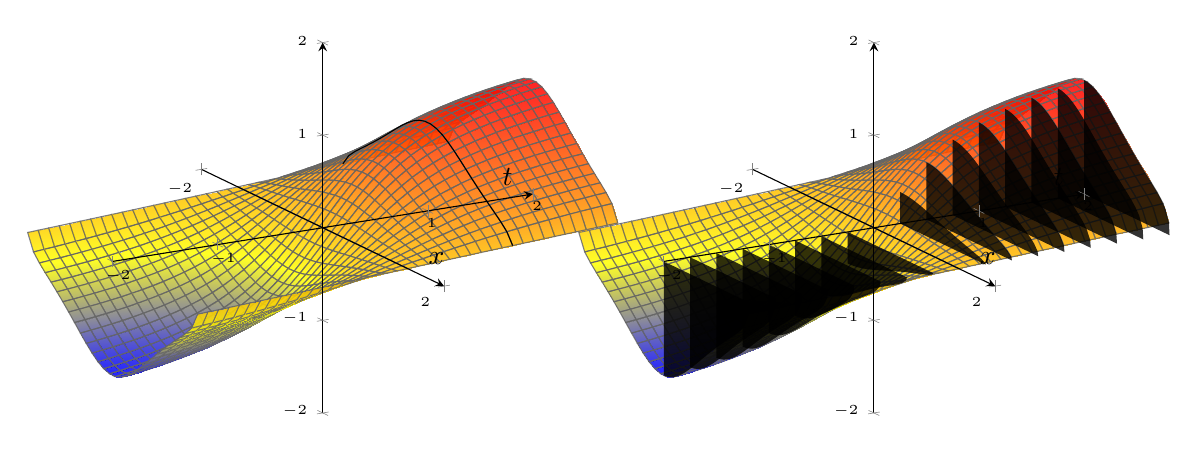
\begin{tikzpicture}[declare function={f(\x,\y)=rad(atan(\y*sqrt(2-\x*\x)))/(1+\x*\x);}]
        \begin{scope}[shift={(7,0)}]
            \begin{axis}[
            axis lines = center,
            axis on top,
            view={60}{20},
            xlabel={$x$}, ylabel={$t$}, zlabel={},
            xmin=-2, xmax=2, ymin=-2, ymax=2,
            zmin=-2, zmax=2,
            tick label style={font=\tiny}
        ]
        \addplot3[
            surf, shader=faceted interp, faceted color=black!60, opacity=0.85,
            samples=30, samples y=41,
            domain=-1.4:1.4, domain y=-2:2,
        ] {f(\x,\y)};

    %     \addplot3[
    % ,domain    = -1.4:1.4
    % ,samples   = 30
    % ,samples y = 1
    % ] ( {x}, {1}, {rad(atan(sqrt(2-x*x)))/(1+x*x)} );

    \pgfplotsinvokeforeach{-2, -1.75,-1.5,-1.25,-1,-0.75,-0.5,-0.25,0,0.25,0.5,0.75,1,1.25,1.5,1.75,2}{\fill[black, opacity=0.8] (0,#1,0) -- plot[variable=\x,domain=0:1.4] (\x,#1,{f(\x,#1)}) -- (1.41,#1,0) --cycle;}
        \end{axis}
        \end{scope}
        \begin{scope}
            \begin{axis}[
            axis lines = center,
            axis on top,
            view={60}{20},
            xlabel={$x$}, ylabel={$t$}, zlabel={},
            xmin=-2, xmax=2, ymin=-2, ymax=2,
            zmin=-2, zmax=2,
            tick label style={font=\tiny}
        ]
        \addplot3[
            surf, shader=faceted interp, faceted color=black!60, opacity=0.85,
            samples=30, samples y=41,
            domain=-1.4:1.4, domain y=-2:2,
        ] {f(\x,\y)};

        \addplot3[
    ,domain    = -1.4:1.4
    ,samples   = 30
    ,samples y = 1
    ] ( {x}, {1}, {rad(atan(sqrt(2-x*x)))/(1+x*x)} );
        \end{axis}
        \end{scope}
    \end{tikzpicture}
\end{center}

Continuing with the technique,

\begin{align*}
    F^\prime(t) &= \frac{\partial}{\partial t}\int_{0}^{\sqrt{2}}{\frac{\arctan{(t\sqrt{2 - x^2})}}{1 + x^2}dx} \\ 
    &= \int_{0}^{\sqrt{2}}{\frac{\partial}{\partial t} \left[\frac{\arctan{(t\sqrt{2 - x^2})}}{1 + x^2}\right]dx} \\
    &= \int_{0}^{\sqrt{2}}{\frac{\sqrt{2-x^2}}{(x^2 + 1)((2-x^2)t^2 + 1)}dx}
\end{align*}

Let $x = \sqrt{2}\sin{\theta} \implies dx = \sqrt{2}\cos{\theta}d\theta$ with bounds $[0, \pi/2]$,

\begin{align*}
    F^\prime(t) &= \int_{0}^{\pi/2}{\frac{\sqrt{2}\cos{\theta}\sqrt{2 - (\sqrt{2}\sin{\theta})^2}}{((\sqrt{2}\sin{\theta})^2 + 1)((2 - (\sqrt{2}\sin{\theta})^2)t^2 + 1)}d\theta} \\
    &= \int_{0}^{\pi/2}{\frac{2\cos^2{\theta}}{(2\sin^2{\theta} + 1)(1 + 2t^2 \cos^2{\theta})}d\theta} \\ 
    &= \evalat*{\left(\frac{\sqrt{6t^2 + 3}\arctan{(\sqrt{3}\tan{\theta})} - \arctan{\left( \frac{\tan{\theta}}{2t^2 + 1} \right)}}{\sqrt{2t^2 + 1}(3t^2 + 1)}\right)}{\theta = \pi/2}_{\theta = 0} \\
    &= \frac{\pi(\sqrt{6t^2 +3} - 1)}{2\sqrt{2t^2 + 1}(3t^2 + 1)}
\end{align*}

Feel free to do the last integral yourself. Finally, to find $F(t)$, we need to integrate $F'(t)$ with respect to $t$.

\begin{align*}
    F(t) &= \frac{\pi}{2}\int{\frac{\sqrt{6t^2 +3} - 1}{\sqrt{2t^2 + 1}(3t^2 + 1)}dt}
\end{align*}

Choosing $t = \frac{\tan u}{\sqrt{2}} \implies dt = \frac{\sec^2{u}}{\sqrt{2}}du$ (which makes $F(t) \implies F(t(u))$ but this is inferred),

\begin{align*}
    \frac{\pi}{2}\int{\frac{\sqrt{6t^2 +3} - 1}{\sqrt{2t^2 + 1}(3t^2 + 1)}dt} &= \frac{\pi}{2}\int{\frac{\sqrt{6\left(\frac{\tan u}{\sqrt{2}}\right)^2 +3} - 1}{\sqrt{2\left(\frac{\tan u}{\sqrt{2}}\right)^2 + 1}\left(3\left(\frac{\tan u}{\sqrt{2}}\right)^2 + 1\right)}\frac{\sec^2{u}}{\sqrt{2}}du} \\ 
    &= \frac{\pi}{2} \int{\frac{\sec{u} (\sqrt{3}\sec{u} - 1)}{3\tan^2{u} + 2}du} \\
    &= \frac{\pi}{2}\left( \arctan{\left(\frac{\sqrt{3}\tan{u}}{\sqrt{2}}\right) - \arctan{\left( \frac{\sin{u}}{\sqrt{2}} \right)}} \right) + C \\ 
    &= \frac{\pi}{2}\arctan{\left( \frac{t(\sqrt{6t^2 + 3} - 1)}{t^2\sqrt{3} + \sqrt{2t^2 + 1}} \right)} + C
\end{align*}

Now, we have our intergral (since the integral is $0$ when $t = 0$ then $F(0) = 0 \implies C = 0$),
$$
F(t) = \int_{0}^{\sqrt{2}}{\frac{\arctan{(t\sqrt{2 - x^2})}}{1 + x^2}dx} = \frac{\pi}{2}\arctan{\left( \frac{t(\sqrt{6t^2 + 3} - 1)}{t^2\sqrt{3} + \sqrt{2t^2 + 1}} \right)}.
$$

Our original integral occurs when $t = 1$, or, $F(1)$. 

\begin{align*}
    F(1) &= \int_{0}^{\sqrt{2}}{\frac{\arctan{(\sqrt{2 - x^2})}}{1 + x^2}dx} \\
    &= \frac{\pi}{2}\arctan{\left( \frac{(\sqrt{6 + 3} - 1)}{\sqrt{3} + \sqrt{2 + 1}} \right)} = \frac{\pi^2}{12}\\
\end{align*}

Following our Feynman diagram from before, this is the path we've followed:

\begin{center}
        \scalebox{1.1}{
            \tikz \graph [grow right sep]{
                x1 [as =$\int_{0}^{\sqrt{2}}{\frac{\arctan{(\sqrt{2 - x^2})}}{1 + x^2}dx}$] -> {x2[as=$\frac{\pi^2}{12}$, red, xshift=65mm], x3[as=$\int_{0}^{\sqrt{2}}{\frac{\arctan{(t\sqrt{2 - x^2})}}{1 + x^2}dx}$, xshift=-50mm] -> x4[as=$\int_{0}^{\sqrt{2}}{\frac{\sqrt{2-x^2}}{(x^2 + 1)((2-x^2)t^2 + 1)}dx}$, xshift=-50mm] -> x5[as=$\frac{\pi(\sqrt{6t^2 +3} - 1)}{2\sqrt{2t^2 + 1}(3t^2 + 1)}$, xshift=-50mm] -> x6[as=$\frac{\pi}{2}\arctan{\left( \frac{t(\sqrt{6t^2 + 3} - 1)}{t^2\sqrt{3} + \sqrt{2t^2 + 1}} \right)} + C$, red, xshift=-50mm]};
                x6 -> x2;
            };
        }
\end{center}

Substituting this value into our original yields, 

\begin{align*}
   \int_{1}^{\sqrt{2}}{\frac{\arctan{\sqrt{2 - x^2}}}{1+x^2}dx} &= \frac{1}{2}\int_{0}^{\sqrt{2}}{\frac{\arctan{\sqrt{2 - x^2}}}{1+x^2}dx} - \frac{\pi^2}{32} \\
   &= \frac{\pi^2}{24} - \frac{\pi^2}{32} = \frac{\pi^2}{96}\\
\end{align*}

So now, we've finally proved that,
$$\boxed{\int_{1}^{\sqrt{2}}{\frac{\arctan{\sqrt{2 - x^2}}}{1+x^2}dx} = \frac{\pi^2}{96}}$$


\section{$I_{1}:$ Ophanim}
$$
I_{1} = \int_{0}^{\infty}{\frac{\arctan^2{x}}{x^2 + 9}dx}
$$

\begin{center}
    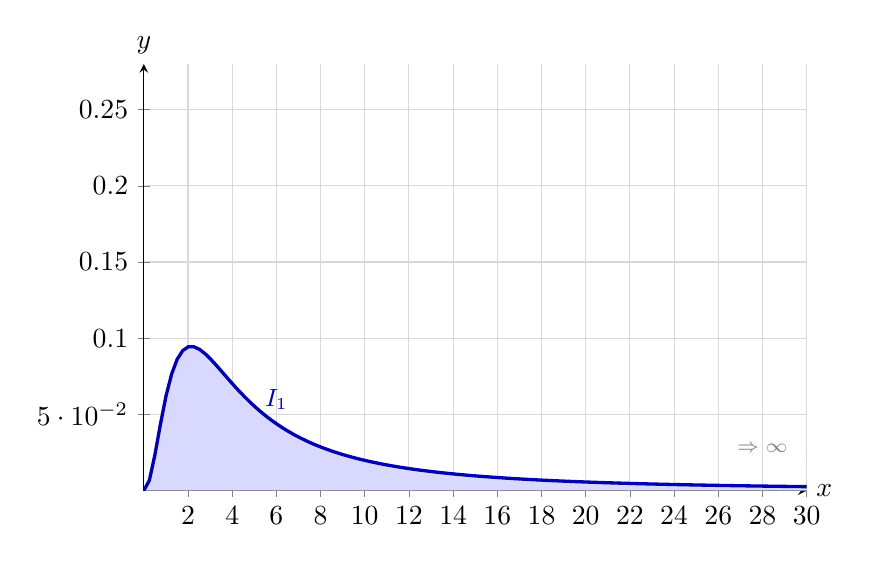
\begin{tikzpicture}

    \begin{axis}[
        width=10cm, height=7cm,
        xmin=0, xmax=30,
        ymin=0, ymax=0.28,
        xlabel={$x$},
        ylabel={$y$},
        axis lines=middle,
        xlabel style={at={(rel axis cs:1,0)}, anchor=west},
        ylabel style={at={(rel axis cs:0,1)}, anchor=south},
        xtick={0,2,4,6,8,10,12,14,16,18,20,22,24,26,28,30},
        ytick={0.05,0.10,0.15,0.20,0.25},
        grid=major,
        grid style={gray!30},
        samples=120,
        domain=0:12,
        every axis plot/.append style={thick},
    ]
    % Shaded area
    \addplot[fill=blue!15, draw=none, domain=0:30] {(rad(atan(x)))^2/(x*x+9)} \closedcycle;
    % Curve
    \addplot[blue!70!black, very thick, domain=0:30] {(rad(atan(x)))^2/(x*x+9)};
    % Label
    \node[blue!70!black, font=\small] at (axis cs:6, 0.06) {$\displaystyle I_1$};
    % Fade arrow suggesting tail to infinity
    \draw[->, thick, gray, dashed] (axis cs:30, 0.023) -- (axis cs:31, 0.019);
    \node[gray, font=\scriptsize] at (axis cs:28, 0.028) {$\Rightarrow\infty$};
    \end{axis}

    \end{tikzpicture}
\end{center}

All methods were unsuccessful, including RIES with the approximation $0.7355031...$ with 100 digits of percision and $80033943411216$ expression searched. So, we'll get right to the evaluation.

Interestingly enough, 
\begin{align*}
    \arctan{(xy)} = \int{\frac{x}{1+y^2 x^2}dy} &\implies \arctan{x} = \int_{0}^{1}{\frac{x}{1+y^2 x^2}dy}\\ &\implies \arctan^2{x} = \int_{0}^{1}{\int_{0}^{1}{\frac{x^2}{(1+y^2 x^2)(1+z^2 x^2)}dydz}}
\end{align*}

So,

\begin{align*}
    \int_{0}^{\infty}{\frac{\arctan^2{x}}{x^2 + 9}dx} &= \int_{0}^{\infty}\frac{1}{x^2 + 9} \left( \int_{0}^{1}{\int_{0}^{1}{\frac{x^2}{(1+y^2 x^2)(1+z^2 x^2)}dydz}} \right)dx \\ 
    &= \int_{0}^{\infty}{\int_{0}^{1}{\int_{0}^{1}{\frac{x^2}{(9+x^2)(1+y^2x^2)(1+z^2x^2)}dydzdx}}}
\end{align*}

If you're familiar with multivariable calculus then you know \textit{Fubini's theorem} which essentially gives you validation that you can swap the order of integration with multiple iterated integrals. \textit{Tonelli’s theorem} is rather similar, except we need the condition that the integrand (the function being integrated) is non-negative (which is clearly the case since $x^2$, $z^2$, $y^2$ are all $>0$) and continous along the bounds $(0, \infty) \times [0, 1]^2$. Analyzing the function across these bounds shows that it is continous, additionally, we could look at the graph of the function. Thus,

\begin{align*}
    \int_{0}^{\infty}{\frac{\arctan^2{x}}{x^2 + 9}dx} &= \int_{0}^{1}{\int_{0}^{1}{\int_{0}^{\infty}{\frac{x^2}{(9+x^2)(1+y^2x^2)(1+z^2x^2)}dxdydz}}}
\end{align*}

The integrand is very nearly in in the form $\frac{x^2}{(x^2 + A^2)(x^2 + B^2)(x^2 + C^2)}$ which would work nicely with partial fraction decomposition. We can easily turn it into such by,

\begin{align*}
    \frac{x^2}{(9+x^2)(1+y^2x^2)(1+z^2x^2)} &= \frac{1}{y^2 z^2}\cdot\frac{x^2}{(x^2 + 9)(x^2 + \frac{1}{y^2})(x^2 + \frac{1}{z^2})} \\ 
    &= (B^2 C^2)\cdot\frac{x^2}{(x^2 + A^2)(x^2 + B^2)(x^2 + C^2)}
\end{align*}

where $A = 3$, $B = \frac{1}{y}$, $C = \frac{1}{z}$. I see a pretty nice generalization here for our integral, specifically,

$$
I_{1}(t) = \int_{0}^{\infty}{\frac{\arctan^2{x}}{x^2 + t^2}dx}.
$$

Which would make $A = t$. Continuing with the decomposition,

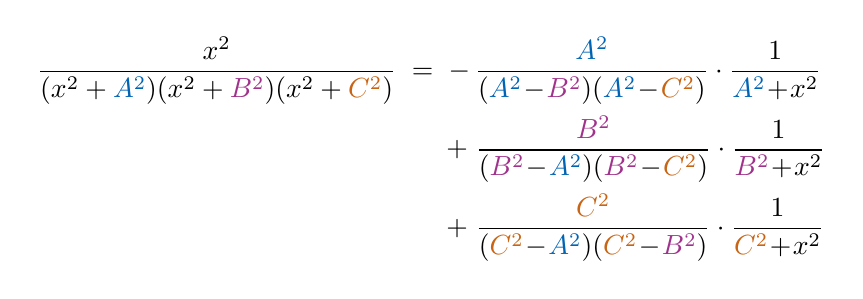
\begin{tikzpicture}
    \node[anchor=west] at (0, 10) {%
$\displaystyle
\frac{x^2}{(x^2+\textcolor{tA}{A^2})(x^2+\textcolor{tB}{B^2})(x^2+\textcolor{tC}{C^2})}
\;=\;
-\,\frac{\textcolor{tA}{A^2}}{(\textcolor{tA}{A^2}\!-\!\textcolor{tB}{B^2})(\textcolor{tA}{A^2}\!-\!\textcolor{tC}{C^2})}
\cdot\frac{1}{\textcolor{tA}{A^2}\!+\!x^2}
$};

    \node[anchor=west] at (5.2, 9.0) {%
    $\displaystyle
    +\;\frac{\textcolor{tB}{B^2}}{(\textcolor{tB}{B^2}\!-\!\textcolor{tA}{A^2})(\textcolor{tB}{B^2}\!-\!\textcolor{tC}{C^2})}
    \cdot\frac{1}{\textcolor{tB}{B^2}\!+\!x^2}
    $};

    \node[anchor=west] at (5.2, 8.0) {%
    $\displaystyle
    +\;\frac{\textcolor{tC}{C^2}}{(\textcolor{tC}{C^2}\!-\!\textcolor{tA}{A^2})(\textcolor{tC}{C^2}\!-\!\textcolor{tB}{B^2})}
    \cdot\frac{1}{\textcolor{tC}{C^2}\!+\!x^2}
    $};
\end{tikzpicture}

Which makes the integral,

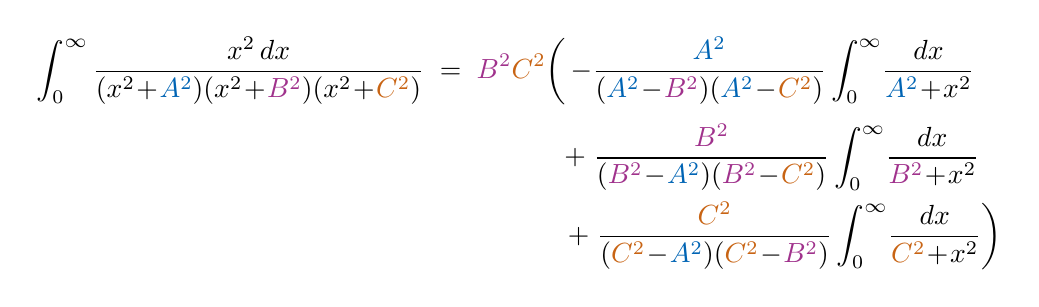
\begin{tikzpicture}
    \node[anchor=west] at (0, 5.5) {%
$\displaystyle
\int_0^\infty \frac{x^2\,dx}{(x^2\!+\!\textcolor{tA}{A^2})(x^2\!+\!\textcolor{tB}{B^2})(x^2\!+\!\textcolor{tC}{C^2})}
\;=\;
\textcolor{tB}{B^2}\textcolor{tC}{C^2}\!\left(\,
-\frac{\textcolor{tA}{A^2}}{(\textcolor{tA}{A^2}\!-\!\textcolor{tB}{B^2})(\textcolor{tA}{A^2}\!-\!\textcolor{tC}{C^2})}
\int_0^\infty\!\frac{dx}{\textcolor{tA}{A^2}\!+\!x^2}
\right.
$};

    \node[anchor=west] at (6.7, 4.4) {%
    $\displaystyle
    +\;\frac{\textcolor{tB}{B^2}}{(\textcolor{tB}{B^2}\!-\!\textcolor{tA}{A^2})(\textcolor{tB}{B^2}\!-\!\textcolor{tC}{C^2})}
    \int_0^\infty\!\frac{dx}{\textcolor{tB}{B^2}\!+\!x^2}
    $};

    \node[anchor=west] at (6.7, 3.4) {%
    $\displaystyle
    \left.
    +\;\frac{\textcolor{tC}{C^2}}{(\textcolor{tC}{C^2}\!-\!\textcolor{tA}{A^2})(\textcolor{tC}{C^2}\!-\!\textcolor{tB}{B^2})}
    \int_0^\infty\!\frac{dx}{\textcolor{tC}{C^2}\!+\!x^2}
    \right)
    $};
\end{tikzpicture}

For any $u \in \mathbb{R}$, $\displaystyle\int_{0}^{\infty}{\frac{1}{x^2 + u^2}dx} = \evalat*{\left( \frac{\arctan{x/u}}{u} \right)}{\infty}_{0} = \frac{\pi}{2u}$, so,

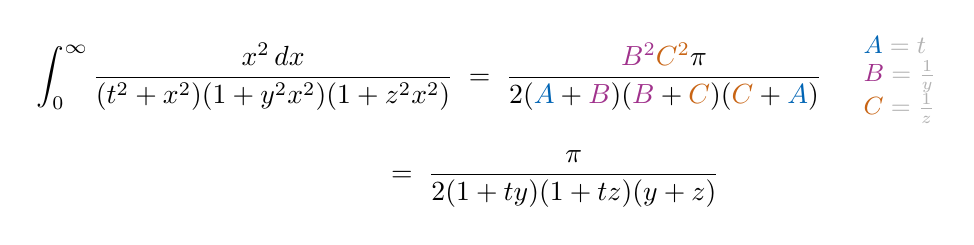
\begin{tikzpicture}
    \node[anchor=west] at (2, 0.5) {%
$\displaystyle
\int_0^\infty \frac{x^2\,dx}{(t^2+x^2)(1+y^2x^2)(1+z^2x^2)}
\;=\;
\frac{\textcolor{tB}{B^2}\textcolor{tC}{C^2}\pi}{2(\textcolor{tA}{A}+\textcolor{tB}{B})(\textcolor{tB}{B}+\textcolor{tC}{C})(\textcolor{tC}{C}+\textcolor{tA}{A})}
$};

    \node[anchor=west, font=\small, gray!60] at (12.5, 0.9) {%
    $\textcolor{tA}{A}=t$};
    \node[anchor=west, font=\small, gray!60] at (12.5, 0.5) {%
    $\textcolor{tB}{B}=\tfrac{1}{y}$};
    \node[anchor=west, font=\small, gray!60] at (12.5, 0.1) {%
    $\textcolor{tC}{C}=\tfrac{1}{z}$};

    \node[anchor=west] at (6.5, -0.8) {%
    $\displaystyle
    =\;\frac{\pi}{2(1+ty)(1+tz)(y+z)}
    $};
\end{tikzpicture}

Substituting back into our original iterated integral ($z = \frac{1}{t}$ is removable),

\begin{align*}
    I_1(t) &= \frac{\pi}{2}\int_{0}^{1}{\int_{0}^{1}{\frac{1}{(1+ty)(1+tz)(y+z)}dydz}} \\ 
    &= \frac{\pi}{2}\left( \int_{0}^{1}{\frac{1}{1 + tz}\left( \int_{0}^{1}{\frac{1}{(1+ty)(y+z)}dy} \right)dz} \right) \\
    &= \frac{\pi}{2}\int_{0}^{1}{\frac{1}{(1+tz)(1-tz)} \ln\left(\frac{1+z}{z(1+t)}\right)dz}
\end{align*}

Typical integral calculators can solve this. However, they yield quite the answer... 
\begin{align*}
    -\frac{1}{2t}\Bigg( \Bigg. &\Li{\frac{2t}{t+1}} - \Li{\frac{t}{t+1}} + \ln^2{(t+1)} + \ln{(t+1)}(-\ln{(|t-1|)} - 2\ln 2) \\& - \Li{\frac{2t}{t-1}} + \Li{\frac{t}{t-1}} - \Li{t} + \Li{-t} + 2\ln 2 \ln{(t-1)} \Bigg. \Bigg)
\end{align*}

($\Li{t}$ will be defined in a moment) but I believe we can do better than this. Let $z = \frac{1-w}{1+w} \implies dz = -\frac{2}{(1+w)^2}dw$ and let $n = \frac{t-1}{t+1}$.

\begin{align*}
    I_1{(t)} &= \frac{\pi}{2} \int_{0}^{1}{\frac{\ln{\left( \frac{1-n}{1-w} \right)}}{\frac{(t+1)^2 (w-n)(1-nw)}{(1+w)^2}} \left( -\frac{2}{(1+w)^2} \right)dw} \\
    &= \frac{\pi(1-n^2)}{4t} \int_{0}^{1}{\frac{\ln{(1-n)} - \ln{(1-w)}}{(w-n)(1-nw)}dw}
\end{align*}

Let's do a bit of Feynman's, let $F(n) = (1-n^2)\int_{0}^{1}{\frac{\ln{(1-n)} - \ln{(1-w)}}{(w-n)(1-nw)}dw}$, we can break it up as

\begin{align*}
    F(n) &= (1-n^2) \int_{0}^{1}{ \left( \frac{1}{w-n} + \frac{n}{1-nw} \right) (\ln{(1-n)} - \ln{(1-w)}) dw} \\
\end{align*}

Let $w = \frac{n + u}{1+nu} \implies dw = \frac{1-n^2}{(1+nu)^2} du$,

\begin{align*}
    F(n) &= \int_{-n}^{1}{\frac{\ln(1 + nu) - \ln(1-u)}{u}du} \\ 
    \implies F'(n) &= \int_{-n}^{1}{\frac{1}{1 + nu}du} \\
    &= \evalat*{\frac{\ln(|nu + 1|)}{n}}{1}_{-n} = -\frac{2\ln(1-n)}{n} \\
    \implies F(n) &= 2\left(-\int{\frac{\ln(1-n)}{n} dn}\right)
\end{align*}

\subsection{Dilogarithm}

The \textbf{polylogarithm} is a special function, denoted as $\text{Li}_{s}(z)$ (for $s\in\mathbb{Z}$ and $z\in\mathbb{C}$), that appears quite frequently in mathematics. It's defined as,

$$
\text{Li}_{s}(z) = \sum_{k=1}^{\infty}{\frac{z^k}{k^s}} = \int_{0}^{z}{\frac{\text{Li}_{(s-1)}(t)}{t}dt}
$$

Notice that for $s = 1$, $\text{Li}_{1}(z) = -\ln(1-z)$. We can then define $\Li{z}$ as

$$
\Li{z} = -\int_{0}^{z}{\frac{\ln(1-t)}{t}dt}.
$$

This function is more commonly known as the \textbf{dilogrithm}. This integral is unsolvable, or, nonelementary (can't be expressed using a finite amount of elementary operation). However, there are some special values of this function as we will come to see. So,

\begin{align*}
    F(n) &= 2\Li{n} + C.
\end{align*}

Clearly if $k = 0$ then $-\int_{0}^{0}{\frac{\ln(1-u)}{u}du} = 0 \implies \Li{0} = 0$, so $C = F(0)$. Recall the definition of a polylogarithm,

\begin{align*}
    F(0) &= -\int_{0}^{1}{\frac{\ln(1-u)}{u}du} \\
    &= \sum_{k=1}^{\infty}{\frac{1}{k^2}} = \frac{\pi^2}{6}
\end{align*}

The last step is a famous result of the Basel Problem. Notice that $-\int_{0}^{1}{\frac{\ln(1-u)}{u}du} = \Li{1} \implies \Li{1} = \pi^2/6$. So,

\begin{align*}
    F(n) &= 2\Li{n} + \frac{\pi^2}{6} \\
    \implies I_1(t) &= \frac{\pi}{4t} \left( 2\Li{\frac{t-1}{t+1}} + \frac{\pi^2}{6} \right) \\
\end{align*}

Our original integral is for $t = 3$, so
\begin{align*}
    I_1(3) &= \int_{0}^{\infty}{\frac{\arctan^2{x}}{x^2 + 9}dx} \\
    &= \frac{\pi}{12} \left( 2\Li{\frac{1}{2}} + \frac{\pi^2}{6} \right).
\end{align*}

Cool enough, we can reduce this further by finding $\Li{\frac{1}{2}}$. It's rather straightforward so I'll showcase it here:
\begin{align*}
    \frac{d}{dx}\left[\Li{1 - x}\right] &= \frac{\ln x}{1-x} \\ 
    \evalat*{\Li{1 - x}}{y}_{0} &= \int_{0}^{y}{\frac{\ln x}{1-x}dx} \\ 
    \Li{1-y} - \Li{1} &= \evalat*{\left(-\ln(1-x)\ln{x}\right)}{y}_{0} + \int_{0}^{y}{\frac{\ln(1-x)}{x}dx} \\
    \Li{1-y} &= \frac{\pi^2}{6}-\ln(1-y)\ln{y} - \Li{y} \\
    \Li{\frac{1}{2}} &= \frac{\pi^2}{12} - \frac{1}{2}\ln^2\left(\frac{1}{2}\right) \\
    &= \frac{\pi^2}{12} - \frac{1}{2}\ln^2(2)
\end{align*}

So, we have

\begin{align*}
    \boxed{\int_{0}^{\infty}{\frac{\arctan^2{x}}{x^2 + 9}dx} = \frac{\pi^3 - 3\pi\ln^2(2)}{36}}
\end{align*}

\section{$I_2$: Gabriel}
$$
\int_{-1}^{1}{\frac{\arcsin{x} + 1}{x\sqrt{1-x^4}} \ln\left( \frac{(x^2 + 1)^{3/2} + x^3}{(x^2 + 1)^{3/2} - x^3} \right)dx}
$$

\begin{center}
    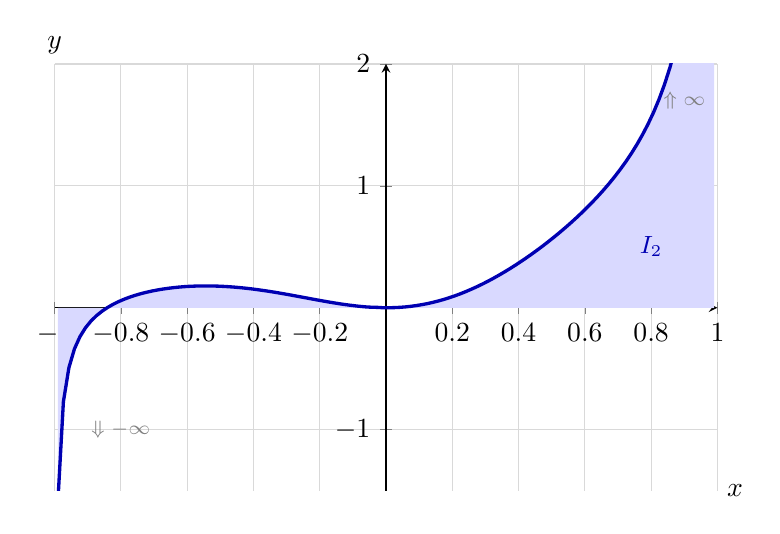
\begin{tikzpicture}

    \begin{axis}[
        width=10cm, height=7cm,
        xmin=-1, xmax=1,
        ymin=-1.5, ymax=2.0,
        xlabel={$x$},
        ylabel={$y$},
        axis lines=middle,
        xlabel style={at={(rel axis cs:1,0)}, anchor=west},
        ylabel style={at={(rel axis cs:0,1)}, anchor=south},
        grid=major,
        grid style={gray!30},
        samples=120,
        domain=0:12,
        every axis plot/.append style={thick},
    ]
    % Shaded area
    \addplot[fill=blue!15, draw=none, domain=-.99:.99] {(rad(asin(x)) + 1)/(x*sqrt(1-x*x*x*x))*ln(((x*x+1)^(3/2) + x*x*x)/((x*x + 1)^(3/2) - x*x*x))} \closedcycle;
    % Curve
    \addplot[blue!70!black, very thick, domain=-.99:.99] {(rad(asin(x)) + 1)/(x*sqrt(1-x*x*x*x))*ln(((x*x+1)^(3/2) + x*x*x)/((x*x + 1)^(3/2) - x*x*x))};
    % Label
    \node[blue!70!black, font=\small] at (axis cs:.8, 0.5) {$\displaystyle I_2$};
    % Fade arrow suggesting tail to infinity
    \node[gray, font=\scriptsize] at (axis cs:.9,1.7) {$\Uparrow\infty$};
    \node[gray, font=\scriptsize] at (axis cs:-.8,-1) {$\Downarrow-\infty$};
    \end{axis}
    \end{tikzpicture}
\end{center}

REIS yields $\pi\arcsin(3 - \sqrt{7})$ as an answer from the numerical value of $1.13760379218104...$ This will be good motivation later on. First let's break this into two integrals from the numerator being $\arcsin{x} + 1$,

$$
I_{2} = \int_{-1}^{1}{\frac{\arcsin{x}}{x\sqrt{1-x^4}} \ln\left( \frac{(x^2 + 1)^{3/2} + x^3}{(x^2 + 1)^{3/2} - x^3} \right)dx} + \int_{-1}^{1}{\frac{1}{x\sqrt{1-x^4}} \ln\left( \frac{(x^2 + 1)^{3/2} + x^3}{(x^2 + 1)^{3/2} - x^3} \right)dx}
$$

The first integral is odd, so it's zero across the bounds $[-1, 1]$. So the integral is now,

$$I_{2} = \int_{-1}^{1}{\frac{1}{x\sqrt{1-x^4}} \ln\left( \frac{(x^2 + 1)^{3/2} + x^3}{(x^2 + 1)^{3/2} - x^3} \right)dx}.$$

Let $x = \tan{t} \implies dx = \sec^2{t}dt$ and $[-1, 1] \to [\pi/4, -\pi/4]$,
\begin{align*}
    I_{2} &= \int_{-\pi/4}^{\pi/4}{\frac{1}{\tan{t}\sqrt{1-(\tan{t})^4}} \ln\left( \frac{((\tan{t})^2 + 1)^{3/2} + (\tan{t})^3}{((\tan{t})^2 + 1)^{3/2} - (\tan{t})^3} \right)\sec^2{t}dt} \\
    &= \int_{-\pi/4}^{\pi/4}{\frac{\cos{t}}{\sin{t}\sqrt{1 - 2\sin^2{t}}} \ln\left( \frac{1 + \sin^3 t}{1 - \sin^3 t} \right) dt} \\
    &= \int_{-\pi/4}^{\pi/4}{\frac{\cos{t}}{\sin{t}\sqrt{1 - 2\sin^2{t}}} \ln\left( 1 + \sin^3 t \right) dt} - \int_{-\pi/4}^{\pi/4}{\frac{\cos{t}}{\sin{t}\sqrt{1 - 2\sin^2{t}}} \ln\left( 1 - \sin^3 t \right) dt}\\
    &= 2\int_{-\pi/4}^{\pi/4}{\frac{\cos{t}}{\sin{t}\sqrt{1 - 2\sin^2{t}}} \ln\left( 1 + \sin^3 t \right) dt}
\end{align*}

Let $u = \sin(t) \implies du = \cos(t)dt$ and $[-\pi/4, \pi/4] \to [-1/\sqrt{2}, 1/\sqrt{2}]$, then, after simplifying, let $u = \sin(w)/\sqrt{2} \implies du = (\cos(w)/\sqrt{2}) dw$ and $[-1/\sqrt{2}, 1/\sqrt{2}] \to [-\pi/2, \pi/2]$

\begin{align*}
    I_{2} &= 2\int_{-1/\sqrt{2}}^{1/\sqrt{2}}{\frac{\ln\left( 1 + u^3 \right)}{u\sqrt{1 - 2u^2}}du} = 2\int_{-\pi/2}^{\pi/2}{\frac{\ln\left( 1 + \left(\frac{\sin w}{\sqrt{2}}\right)^3 \right)}{\sin{w}}dw}
\end{align*}

If we can split $\left(\frac{\sin w}{\sqrt{2}}\right)^3$ into three products, then we can split the integral into three parts. There are no ifs in this case, this is exactly what we are going to do. Using roots of unity, $1 + x^3$ has zeros at $x = -1, e^{\frac{\pi i}{3}}, e^{-\frac{\pi i}{3}}$, so,

\begin{align*}
    I_{2} &= 2\left( \int_{-\pi/2}^{\pi/2}{\frac{\ln\left( 1 + \frac{\sin{w}}{\sqrt{2}} \right)}{\sin{w}}dw} + \int_{-\pi/2}^{\pi/2}{\frac{\ln\left( e^{\frac{\pi i}{3}} + \frac{\sin{w}}{\sqrt{2}} \right)}{\sin{w}}dw} + \int_{-\pi/2}^{\pi/2}{\frac{\ln\left( e^{\frac{-\pi i}{3}} + \frac{\sin{w}}{\sqrt{2}} \right)}{\sin{w}}dw} \right) \\
    &= 2\left( \int_{-\pi/2}^{\pi/2}{\frac{\ln\left( 1 + \frac{1}{\sqrt{2}}\sin{w} \right)}{\sin{w}}dw} + \int_{-\pi/2}^{\pi/2}{\frac{\ln\left( 1 - \frac{e^{\frac{\pi i}{3}}}{\sqrt{2}}\sin{w} \right)}{\sin{w}}dw} + \int_{-\pi/2}^{\pi/2}{\frac{\ln\left( 1 - \frac{e^{\frac{-\pi i}{3}}}{\sqrt{2}}\sin{w} \right)}{\sin{w}}dw} \right) \\
\end{align*}

We'll solve the general case,

\begin{align*}
    F(b) &= \int_{-\pi/2}^{\pi/2}{\frac{\ln\left( 1 + b\sin{w} \right)}{\sin{w}}dw} \\
    \implies F^\prime(b) &= \int_{-\pi/2}^{\pi/2}{\frac{1}{b\sin w + 1}dw} \\
\end{align*}

To solve this integral, we'll use Weierstrass Substitution (or Tangent half-angle substitution). First, let $t = \tan{\frac{w}{2}}$ which then makes $\sin{w} = \frac{2t}{1+t^2}$, $\cos{w} = \frac{1-t^2}{1+t^2}$, and $dw = \frac{2 dt}{1+t^2}$. The bounds are thus $[\pi/2, -\pi/2] \to [1, -1]$. Note, we can only use Weierstrass Substitution when we have a rational function in terms of trigonometric functions. 

\begin{align*}
    F^\prime(b) &= \int_{-1}^{1}{\frac{1}{b\left( \frac{2t}{1+t^2} \right) + 1} \left( \frac{2}{1+t^2} \right)dt} \\
    &= \int_{-1}^{1}{\frac{2}{t^2 + 2bt - 1}dt} = 2\int_{-1}^{1}{\frac{1}{(t + b)^2 + (\sqrt{1 - b^2})} dt} \\
    &= \frac{2}{\sqrt{1-b^2}}\evalat*{\left(\arctan\left(\frac{t + b}{\sqrt{1 - b^2}} \right)\right)}{1}_{-1} \\
    &= \frac{2}{\sqrt{1 - b^2}}\left( \arctan\left(\frac{b + 1}{\sqrt{1 - b^2}} \right) - \arctan\left(\frac{b - 1}{\sqrt{1 - b^2}} \right) \right)
\end{align*}

Note that $\frac{b + 1}{\sqrt{1 - b^2}} = -\left(\frac{b - 1}{\sqrt{1 - b^2}} \right)^{-1}$ and $\arctan{x} + \arctan{\frac{x}{2}} = \frac{\pi}{2}$ for $x > 0$. So,

\begin{align*}
    F^\prime(b) &= \frac{2}{\sqrt{1-b^2}}\cdot \frac{\pi}{2} = \frac{\pi}{\sqrt{1 - b^2}} \\
    \implies F(b) &= \pi\int{\frac{1}{\sqrt{1 - b^2}}db} \\
    &= \pi\arcsin{b} + C
\end{align*}

When $F(0) = \int_{-\pi/2}^{\pi/2}{0dw} = 0 \implies C = 0$. So,
$$
\int_{-\pi/2}^{\pi/2}{\frac{\ln\left( 1 + b\sin{w} \right)}{\sin{w}}dw} = \pi\arcsin{b}.
$$

Using this result, we turn back to $I_2$,

\begin{align*}
    I_{2} &= 2\left( \int_{-\pi/2}^{\pi/2}{\frac{\ln\left( 1 + \frac{1}{\sqrt{2}}\sin{w} \right)}{\sin{w}}dw} + \int_{-\pi/2}^{\pi/2}{\frac{\ln\left( 1 - \frac{e^{\frac{\pi i}{3}}}{\sqrt{2}}\sin{w} \right)}{\sin{w}}dw} + \int_{-\pi/2}^{\pi/2}{\frac{\ln\left( 1 - \frac{e^{\frac{-\pi i}{3}}}{\sqrt{2}}\sin{w} \right)}{\sin{w}}dw} \right) \\
    &= 2\pi\arcsin{\frac{1}{\sqrt{2}}} - 2\pi\arcsin{\frac{e^{-\frac{\pi i}{3}}}{\sqrt{2}}} - 2\pi\arcsin{\frac{e^{\frac{\pi i}{3}}}{\sqrt{2}}} \\
    &= \frac{\pi^2}{2} -2\pi\left( \arcsin{\frac{e^{-\frac{\pi i}{3}}}{\sqrt{2}}} - \arcsin{\frac{e^{\frac{\pi i}{3}}}{\sqrt{2}}} \right)
\end{align*}

This may seem to be a complete solution at first, but remember our solution from RIES. We will continue with the evaluation. For some $x, y \in \mathbb{C}$ such that $|x^2 + y^2| \leq 1$, we have $\arcsin{x} + \arcsin{y} = \arcsin{\left( x\sqrt{1 - y^2} +y\sqrt{1 - x^2} \right)}$. So we can write,
\begin{align*}
    I_{2} &= \frac{\pi^2}{2} -2\pi\left( \arcsin{\frac{e^{-\frac{\pi i}{3}}}{\sqrt{2}}} - \arcsin{\frac{e^{\frac{\pi i}{3}}}{\sqrt{2}}} \right) \\
    &= \frac{\pi^2}{2} - 2\pi\arcsin\left( \frac{\sqrt{\sqrt{28} + 5}-\sqrt{3}\sqrt{\sqrt{28} - 5}}{4} \right)
\end{align*}

We can attempt to simplify the expression inside $\arcsin$. Let's try and get it in the form of $\sqrt{x + \sqrt{y}}$.

\begin{align*}
    \sqrt{x + \sqrt{y}} &= \frac{\sqrt{\sqrt{28} + 5}-\sqrt{3}\sqrt{\sqrt{28} - 5}}{4} \\
    x + \sqrt{y} &= \frac{\left(\sqrt{\sqrt{28} + 5}-\sqrt{3}\sqrt{\sqrt{28} - 5}\right)^2}{2} \\
    &= \frac{\sqrt{28} - 4}{4} \\ 
    \implies  \frac{1}{2}\sqrt{\sqrt{28}-4} &= \frac{\sqrt{\sqrt{28} + 5}-\sqrt{3}\sqrt{\sqrt{28} - 5}}{4}
\end{align*}

Next, as a corollary to the earlier $\arcsin$ identity, it can be shown that $2\arcsin{x} = \arcsin{\sqrt{2x\sqrt{1-x^2}}}$, so,

\begin{align*}
    I_{2} &= \pi \left( \frac{\pi}{2} - 2\arcsin\left( \frac{1}{2}\sqrt{\sqrt{28}-4} \right)\right) \\
    &= \pi \left( \frac{\pi}{2} - \arcsin\left(\sqrt{\sqrt{28}-4}\sqrt{1 - \left( \sqrt{\sqrt{28}-4}\right)^2}  \right) \right) \\ 
    &= \pi \left( \frac{\pi}{2} - \arcsin\left( \frac{\sqrt{12\sqrt{28} - 60}}{2} \right) \right)
\end{align*}

We'll once again use the $\arcsin$ identity but with $\pi / 2 = \arcsin{1}$, so, 
\begin{align*}
    I_{2} &= \pi \left( \arcsin{1} -  \arcsin\left( \frac{\sqrt{12\sqrt{28} - 60}}{2} \right) \right) \\ 
    &= \pi\arcsin\left( \sqrt{1 - \left( \frac{\sqrt{12\sqrt{28} - 60}}{2}\right)^2} \right) \\
    &= \pi \arcsin \left( \sqrt{16 - 6\sqrt{7}} \right)
\end{align*}

We're just about finished, we just have to represent $\sqrt{16 - 6\sqrt{7}}$ as $x - \sqrt{y}$ (based on the result we got using RIES),

\begin{align*}
    \sqrt{16 - 6\sqrt{7}} &= x - \sqrt{y} \\
    16 - 6\sqrt{7} &= x^2 + y - 2x\sqrt{y} \\ 
    \implies x = 3, y = 7 &\implies \sqrt{16 - 6\sqrt{7}} = 3 - \sqrt{7}
\end{align*}

So, finally,

$$
\boxed{\int_{-1}^{1}{\frac{\arcsin{x} + 1}{x\sqrt{1-x^4}} \ln\left( \frac{(x^2 + 1)^{3/2} + x^3}{(x^2 + 1)^{3/2} - x^3} \right)dx} = \pi\arcsin\left(3 - \sqrt{7}\right)}
$$

\end{document}